\chapter{Ewaluacja aplikacji}

\section{Cel}
Celem badania jest poznanie zdania prawdziwych użytkowników.
\section{Plan badania}
Aplikacja zostanie przedstawiona zespołowi,
który tworzy oprogramowanie z wykorzystaniem metodyk zwinnych.
Jako że członkowie zespołu po usłyszeniu założeń projektu, stwierdzili,
że nie chcą aby aplikacja ewentualnia zniszczyła któryś z ich projektów,
a sami nie chcą tworzyć nowych historyjek stwierdziliśmy,
że w ramach testu stworzę testowe issues.
Dlatego właśnie autor aplikacji będzie scrum masterem a badani będą graczami,
więc będą oceniać historyjki.
Jako że aplikacja jest podobna do funkcjonujących na rynku,
nie trzeba było zbytnio badanym objaśnień działania aplikacji.
Badanie będzie wykonane przy skali Fibunacciego,
karty będą automatycznie odkrywane gdy wszyscy zagłosowali.
 Aplikacja będzie obliczała sama końcową ocenę a scrum master nie będzie głosował.
 \textbf{Nazwa badania}: Planning poker
 \textbf{Backlog}: Saving games to database, Filter issues, Adding list to database,
 Implementation of gameplay, Interface for game, connecting planning poker to firebase,
implementation of game cards, adding create game form, integration with github.
\section{Wyniki}
Przebadani użytkownicy mieli pod przewodnictwem autora ocenić 10 testowych historyjek.
Mieli oni korzystać z czterech różnych przeglądarek.
Badanie trwało 10 min. po których użytkownicy mieli wypełnić ankietę i dodać ewentualne uwagi.
~\ref{rys:wynikBadania}
\begin{figure}[H]
	\centering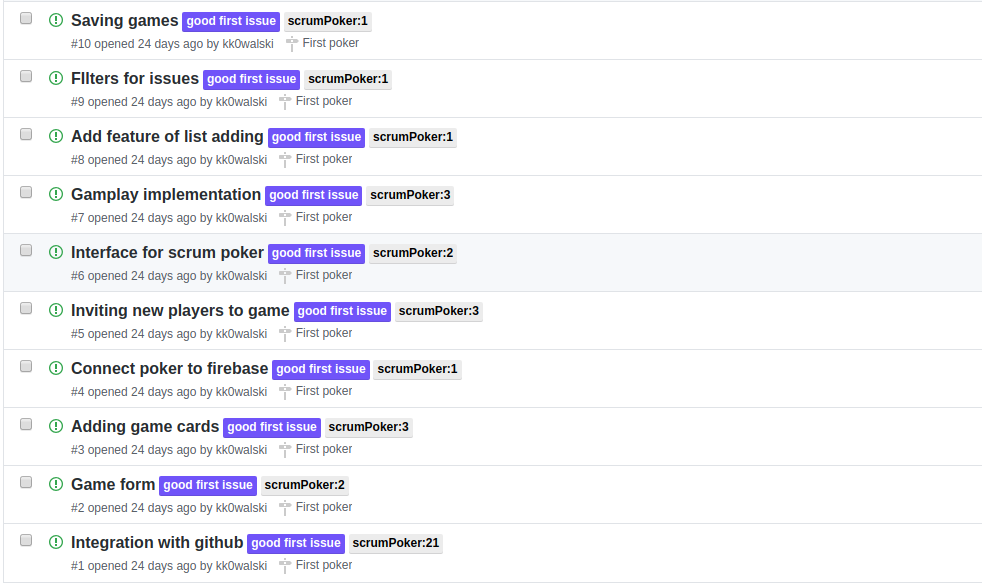
\includegraphics[width=.9\textwidth]{img/wynikBadania}
	\caption{Ocenione historyjki w Github'ie}.
	\label{rys:wynikBadania}
\end{figure}

